\documentclass[12pt,letterpaper]{article}
\usepackage[utf8]{inputenc}
\usepackage{amsmath,amssymb,fullpage,graphicx}
\usepackage{subfigure}
\let\hat\widehat
\let\tilde\widetilde


\author{Nan Tang\\1662478}
	%% your name
\title{STAT 403 Spring 2018\\HW04}
	%% title of this document
\begin{document}
\maketitle
	%% make the title and author

\section*{Q1}

\subsection*{Q1-a}
\begin{align*}
Bias(\bar{X}_n) &= \mathbb{E}(\bar{X}_n) - \lambda \\
&= \mathbb{E}(\frac{\sum_{i=1}^{100}X_i}{100}) - \lambda \\
&= \frac{\sum_{i=1}^{100}(\mathbb{E}(X_i))}{100} - \lambda \\
&= \frac{\sum_{i=1}^{100}\lambda}{100} - \lambda \\
&= 0
\end{align*}

\begin{align*}
Var(\bar{X}_n) &= Var(\frac{\sum_{i=1}^{100}X_i}{100}) \\
&= \frac{\sum_{i=1}^{100}Var(X_i)}{100^2} \\
&= \frac{\sum_{i=1}^{100} \lambda}{100^2} \\
&= \frac{\lambda}{100}
\end{align*}

\noindent $X_i \sim Po(\lambda = 4)$, $Var(\bar{X}_n) = \frac{4}{100}$, $Bias(\bar{X}_n) = 0$

\newpage
\subsection*{Q1-b}
\begin{align*}
SE(\bar{X}_n) &= \sqrt[]{Var(\bar{X}_n)} \\
&= \sqrt[]{\frac{\lambda}{100}}
\end{align*}

\noindent $\hat{\lambda} = \bar{X}_n$ is consistent in estimating $\lambda$, and sample size is large enough, thereby we can consider SE as 
\begin{align*}
SE(\bar{X}_n) = \sqrt[]{\frac{\bar{X}_n}{100}}
\end{align*}
\noindent By CLT, $\bar{X}_100$ follows approximately normal distribution with $\mu = \lambda$ and $\sigma = SE(\bar{X}_n)$
\begin{align*}
P(-c \leq \bar{X}_n \leq c) &= 0.9 \\
P(-\frac{c - \lambda}{SE} \leq \frac{\bar{X}_n - \lambda}{SE} \leq  \frac{c - \lambda}{SE}) &= 0.9 \\
P(-\frac{c - \lambda}{SE} \leq  Z  \leq  \frac{c - \lambda}{SE}) &= 0.9 \\
\frac{c - \lambda}{SE} &= Z_{1-\frac{\alpha}{2}} \approx 1.64 \\
P(-1.64 \leq \frac{\bar{X}_n - \lambda}{SE} \leq 1.64) &= 0.9 \\
P(\bar{X}_n -1.64 \cdot SE \leq \lambda \leq \bar{X}_n + 1.64 \cdot SE) &= 0.9 \\
P(\bar{X}_n - 1.64 \cdot \sqrt[]{\frac{\bar{X}_n}{100}} \leq \lambda \leq \bar{X}_n + 1.64 \cdot \sqrt[]{\frac{\bar{X}_n}{100}}) &= 0.9
\end{align*}

\noindent Here we get the $90 \%$ confidence interval for $\lambda$, 
\begin{align*}
CI & = [\bar{X}_n - 1.64 \cdot \frac{\sqrt[]{\bar{X}_n}}{10}, \bar{X}_n + 1.64 \cdot \frac{\sqrt[]{\bar{X}_n}}{10} ]
\end{align*}

\newpage
\subsection*{Q1-c}
\begin{verbatim}
po4_dt <- rpois(100, 4)

hist(po4_dt, main='Histogram of Poisson(4)', probability = T, xlab='X Value', 
     ylab='Density', col='orange')

lambda_est <- mean(po4_dt)
> lambda_est
[1] 4.24
\end{verbatim}

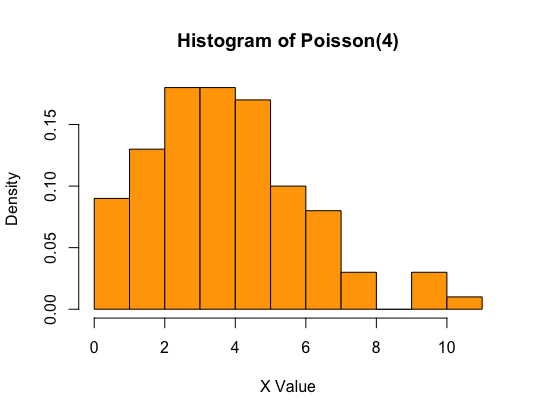
\includegraphics[width=150mm]{hist_po4.png}

\noindent In this scenarios, MLE is equal to 4.24

\newpage
\subsection{Q1-d}
\begin{verbatim}
sim_size <- 10000
sim_result <- rep(NA, sim_size)

for (i in 1:sim_size) {
  po_dt <- rpois(100, 4)
  sim_result[i] <- mean(po_dt)
}

norm_base <- seq(3.0, 5.0, 0.01)
norm_dt <- dnorm(norm_base, 4, 0.2)

hist(sim_result, probability = T, breaks=30, col='darkolivegreen1', 
     main='Histogram of Monte Carlo Poisson(4)', xlab='MLE value', ylab='Density')
lines(norm_base, norm_dt, lwd=2, col='deepskyblue')
\end{verbatim}

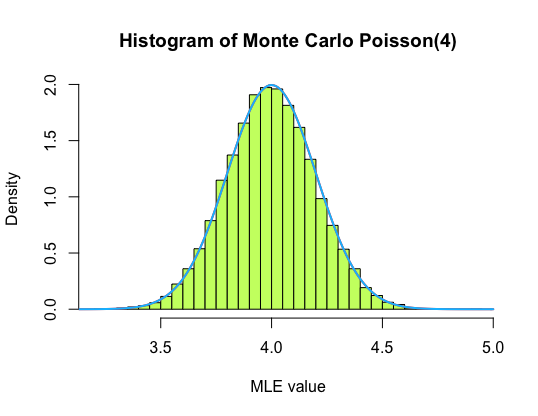
\includegraphics[width=150mm]{hist_mc.png}

\noindent The distribution of simulated MLE fits the normal curve $N(4, 0.2^2)$.

\newpage
\subsection*{Q1-e}

\begin{verbatim}
> sum(sim_result >= 3.5 & sim_result <= 4.5) / sim_size
[1] 0.9876
\end{verbatim}

\noindent Among 10000 simulations, 9876 of them fell in the interval $[3.5, 4.5]$, the fraction is $0.9876$. \\

\noindent From previous part, we perceived that the distribution of MLE follows a normal distribution. The mean of this distribution is equal to $\lambda = 4$, since $\lambda_{MLE}$ is an unbiased estimator for $lambda$. The variance of MLE is, as we calculated in problem a, $\frac{4}{100}$. The distribution of $\lambda_{MLE}$ turns out to be $Normal(4, 0.04)$.\\

\noindent The proportion of simulated MLE that falls into the interval $[3.5, 4.5]$ can be represented by 
\begin{align*}
P(3.5 \leq \lambda_{MLE} \leq 4.5) &= P(\frac{3.5 - \mathbb{E}(\lambda_{MLE})}{SE(\lambda_{MLE})} \leq Z \leq \frac{4.5 - \mathbb{E}(\lambda_{MLE})}{SE(\lambda_{MLE})}) \\
&= P(\frac{3.5-4}{0.2} \leq Z \leq \frac{4.5-4}{0.2}) \\
&= \Phi(2.5) - \Phi(-2.5) \\
&\approx 0.9876
\end{align*}

\newpage
\subsection*{Q2-a}
\begin{verbatim}
quakes <- read.table('fijiquakes.dat', sep='', header=T)

hist(quakes$stations, probability=T, main='Histogram of EarthQuake Stations',
     xlab='Stations', col='skyblue')
\end{verbatim}

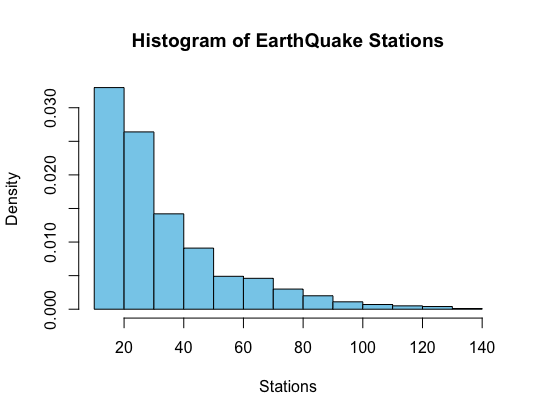
\includegraphics[width=150mm]{hist_station.png}

\newpage
\subsection*{Q2-b}
\noindent The MLE for $\lambda$ for exponential distribution is $\frac{n}{\sum_{i=1}^{n}X_i} = \frac{1}{\bar{X}_n}$, so we choose $\frac{1}{\bar{X}_n}$ as fitted value for ratio parameter.

\begin{verbatim}
lambda_est <- 1/mean(quakes$stations)
> lambda_est
[1] 0.02992399
\end{verbatim}

\noindent The estimated ration parameter is 0.02992

\begin{verbatim}
exp_base <- seq(10, 140, 0.01)
exp_dt <- dexp(exp_base, lambda_est)

hist(quakes$stations, probability=T, main='Histogram of EarthQuake Stations',
     xlab='Stations', col='cadetblue1')
lines(exp_base, exp_dt, lwd=2, col='chocolate1')
legend('topright', legend=('Exp(0.02992)'), col='chocolate', lwd=3, cex=0.75)
\end{verbatim}

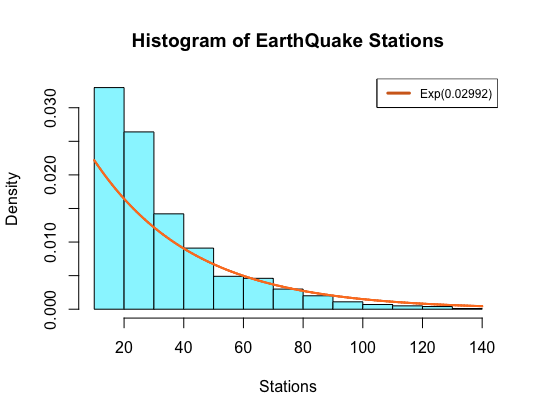
\includegraphics[width=150mm]{hist_exp.png}

\noindent Both station distribution and the exponential distribution skew to right. However, station's distribution seems to be denser on the right tail.  

\newpage
\subsection*{Q2-c}
\begin{verbatim}
linear_reg = lm(quakes$mag~quakes$stations)
> summary(linear_reg)$coeff[2,1]
[1] 0.01565421
\end{verbatim}

\noindent The linear model of mag versus stations has a slope of 0.0157.

\begin{verbatim}
plot(x=quakes$stations, y=quakes$mag, pch=19, cex=0.8, col='gray50', xlab='Station',
     ylab='Magnitude', main='Scatter Plot of Mag VS Station')
abline(linear_reg, lwd=3, col='skyblue')
legend('bottomright', legend=('Fitted Linear Curve'), col='skyblue', lwd=3, cex=0.75)
\end{verbatim}

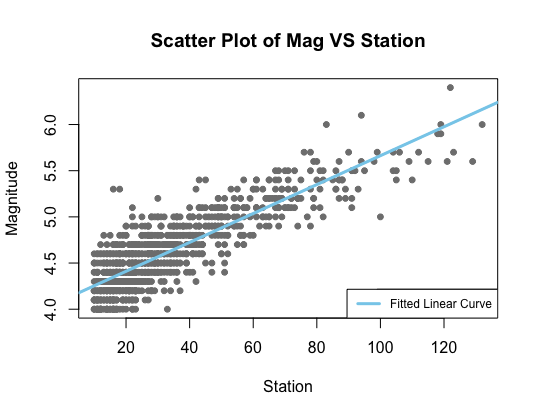
\includegraphics[width=150mm]{scatter_linear.png}

\newpage
\subsection*{Q2-d}
\noindent The $95 \%$ confidence interval of fitted slope $\beta_1$ is 
\begin{align*}
[\hat{\beta_1} - Z_{0.975} \cdot sd(\hat{\beta_1}), \hat{\beta_1} + Z_{0.975} \cdot sd(\hat{\beta_1}) ]
\end{align*}

\begin{verbatim}
beta1 <- summary(linear_reg)$coeff[2,1]
sd_beta1 <- summary(linear_reg)$coeff[2,2]
lowerbd <- beta1 - qnorm(0.975) * sd_beta1
upperbd <- beta1 + qnorm(0.975) * sd_beta1
> c(lowerbd, upperbd)
[1] 0.01505533 0.01625310
\end{verbatim}

\noindent The $95 \%$ CI of fitted slope is $[0.01505533, 0.01625310]$.

%%% do not touch anything below
\end{document}
